\documentclass[conference]{IEEEtran}
\IEEEoverridecommandlockouts
\usepackage[T1]{fontenc}
\usepackage{cite}
\usepackage{amsmath,amssymb,amsfonts}
\usepackage{algorithm}
\usepackage{algorithmic}
\usepackage{graphicx}
\usepackage{textcomp}
\usepackage{xcolor}
\usepackage{booktabs}
\usepackage{multirow}
\usepackage{makecell}
\usepackage{url}
\usepackage{orcidlink}

\def\BibTeX{{\rm B\kern-.05em{\sc i\kern-.025em b}\kern-.08em
    T\kern-.1667em\lower.7ex\hbox{E}\kern-.125emX}}

\begin{document}

\title{Metaheuristic-Driven Client Selection for Federated Android Malware Classification under Non-IID Data Distribution}

\author{\IEEEauthorblockN{Derara Senay Shanka\,\orcidlink{0009-0002-2956-2616} and Peter Shaojui Wang\,\orcidlink{0000-0001-6785-7912}}
\IEEEauthorblockA{Department of Computer Science and Information Engineering\\
National Taiwan University of Science and Technology, Taipei 106, Taiwan\\
Email: derjan06@gmail.com; shaojuiwang@gmail.com}}

\maketitle

\begin{abstract}
Existing federated learning (FL) client-selection methods such as Oort and Power-of-Choice score clients individually and fail to account for the collective diversity of the selected subset, causing convergence failures under severe non-IID data distributions. We propose a combinatorial client-selection framework that scores entire candidate subsets using a three-term composite fitness function capturing model divergence, class-distribution coverage, and pairwise inter-client diversity, solved via metaheuristic search over a large combinatorial space. Evaluated on CCCS-CIC-AndMal-2020 under severe Dirichlet non-IID partitioning across 20 clients classifying 12 malware families, the Aquila Optimizer (AO) instantiation achieves 85.14\% peak F1-macro with zero convergence failures across 15 independent seeds (Grey Wolf Optimizer reaches 85.33\%, a non-significant difference, $p=0.127$), compared to 3/15 failures for Oort and 3/15 for Power-of-Choice; a 12.2\% reduction in mean rounds-to-82\% against Oort (all 15 seeds, non-converging capped at 50), with effect sizes of $d=0.77$ (Oort, approaching large) and $d=0.44$ (PoCo, approaching medium). Validation across three structurally distinct metaheuristic instantiations (Aquila Optimizer, Grey Wolf Optimizer, Particle Swarm Optimization) of the identical fitness function confirms that improvements are attributable to the fitness-function formulation rather than the specific optimizer. An ablation study suggests divergence as the likely primary contributing term, though results are non-significant at $n=15$.
\end{abstract}

\begin{IEEEkeywords}
Federated Learning, Client Selection, Metaheuristic Optimization, Aquila Optimizer, Android Malware Detection, Non-IID Data
\end{IEEEkeywords}

\section{Introduction}

Federated Learning (FL) \cite{mcmahan2017} enables privacy-preserving Android malware detection without centralizing device data, but introduces two compounding challenges: the malware family distribution across devices is highly non-IID, and bandwidth and availability constraints require selecting only a subset of $k$ clients per round \cite{bonawitz2019scale}. The central question is: \emph{which subset should be selected?}

Existing methods such as Oort \cite{lai2021oort} and Power-of-Choice (PoCo) \cite{cho2022poco} assign a scalar utility score to each client and select the top-$k$ independently. This per-client scoring fundamentally cannot capture \emph{collective} subset properties: individually high-utility clients may still be redundant if they share similar local class distributions, leaving the global model blind to absent malware families \cite{balakrishnan2022divfl}.

We reformulate client selection as a \emph{combinatorial subset-level scoring} problem. A three-term composite fitness function scores entire candidate subsets on model-weight divergence, class-distribution coverage, and pairwise inter-client diversity. Because exhaustive search over all $\binom{n}{k}$ subsets is intractable, we solve it via metaheuristic search, instantiated with three structurally distinct optimizers (AO \cite{abualigah2021aquila}, GWO \cite{mirjalili2014gwo}, PSO \cite{kennedy1995pso}) to verify that performance is attributable to the fitness function, not to any specific optimizer. Experiments are conducted on CCCS-CIC-AndMal-2020 across 20 clients under Dirichlet Dir(0.1) non-IID partitioning, a substantially harder setting than prior FL malware detection work (Section~II-B).

Our contributions are:
\vspace{-4pt}
\begin{itemize}
\setlength{\itemsep}{0pt}\setlength{\parskip}{0pt}
\item A subset-level combinatorial fitness function capturing collective divergence, class coverage, and pairwise diversity, achieving zero convergence failures across 15 seeds; ablation suggests divergence as the likely primary contributing term (non-significant at $n=15$).
\item Validation across three metaheuristic instantiations (AO, GWO, PSO) of the identical fitness function, isolating the formulation rather than the optimizer as the source of improvement.
\item Statistically significant convergence improvements over Oort and PoCo across 15 seeds (paired Wilcoxon, $p<0.05$); AO's zero-failure reliability is sustained across $k\in\{6,\dots,12\}$, with significant improvement over Oort at $k=12$ ($p=0.031$).
\end{itemize}
\vspace{-4pt}

\section{Related Work}

Android malware detection has been studied through static, dynamic, and hybrid analysis paradigms \cite{smmarwar2024review}. Centralized approaches on datasets such as CCCS-CIC-AndMal-2020 report strong results using dynamic runtime features, but assume all training data is centrally available, an assumption incompatible with on-device privacy constraints. This motivates the two bodies of work most relevant to the present paper: FL-based malware detection and FL client selection.

\subsection{Federated Learning for Android Malware Detection}
Fang et al.\ \cite{fang2023fedriod} proposed FEDroid, integrating genetic-algorithm-based malware variant augmentation with a residual-network classifier under FL \cite{mcmahan2017}, reporting 98.53\% weighted F1 in cross-dataset evaluation. However, FEDroid assumes IID client data (noted as a limitation by the authors) and treats detection as binary classification with only 3--7 clients. The present work instead evaluates under severe Dir(0.1) non-IID partitioning across 20 clients with 12 distinct malware families.

\subsection{Client Selection in Federated Learning}
Several methods address the client-selection problem in FL \cite{li2024survey}. Oort \cite{lai2021oort} combines statistical and system utility into a per-client scalar score. Power-of-Choice \cite{cho2022poco} biases selection toward higher-loss clients sampled from a candidate pool. Both are per-client scoring approaches. DivFL \cite{balakrishnan2022divfl} instead selects diverse client subsets via submodular maximization, targeting collective subset properties rather than individual utility. FedDiverse \cite{nemeth2025feddiverse} similarly selects subsets with complementary heterogeneity profiles; clients share a compact three-scalar heterogeneity triplet (class-imbalance, attribute-imbalance, and spurious-correlation scores), and it has been validated on computer-vision benchmarks only. FedCor \cite{tang2022fedcor} models inter-client loss correlations via a Gaussian Process, while FAVOR \cite{wang2020favor} trains a deep Q-network to counteract non-IID skew. Zhang et al.\ \cite{zhang2023dpp} apply determinantal point process (DPP) sampling to FL client selection, choosing subsets with probability proportional to $\det(L_S)$, a collective set-function that implicitly penalizes redundant clients; this approach targets computer-vision benchmarks and does not employ metaheuristic search.

\subsection{Metaheuristic Optimization in Federated Learning}
Metaheuristic algorithms have been applied to FL primarily for hyperparameter and model-weight optimization rather than client selection. Qolomany et al.\ \cite{qolomany2020psofl} applied PSO to optimize local-model hyperparameters in an FL setting for smart-city and IoT services. More recently, Yamany et al.\ \cite{yamany2024gwofl} proposed GWOFL, employing Grey Wolf Optimization to generate personalized initial local models for each client, thereby improving robustness against data-poisoning adversarial attacks under non-IID conditions. Critically, both works apply swarm-intelligence optimization \emph{within} the local training or aggregation pipeline, not to the problem of \emph{which clients to select} each round. Two more recent works do target the client-selection step with SI: Khan and Goodridge \cite{khan2024swarm} evaluate nine SI algorithms for FL client selection in cybersecurity scenarios, while Ben Driss et al.\ \cite{bendriss2024gwo} apply GWO to multi-attribute client selection in over-the-air (OTA) FL, balancing accuracy, energy, delay, and fairness. However, both score \emph{individual} clients on a weighted utility function and select the top-$k$, an architecture equivalent to Oort that does not model collective subset properties such as class-distribution coverage or inter-client diversity. FedCSGA \cite{wu2025fedcsga} and FedGenBlk \cite{panimalar2026fedgenblk} apply GAs to client selection but optimize objectives that decompose additively across clients---a deadline-constrained accuracy sum for FedCSGA, and a per-client composite of accuracy, gradient deviation, and blockchain-verified credibility for FedGenBlk---and therefore capture no inter-client statistical structure such as class coverage or pairwise distribution distances.

\subsection{Research Gap}
As Table~\ref{tab:relwork} shows, prior metaheuristic client-selection methods---Khan \& Goodridge, Ben Driss et al., FedCSGA, and FedGenBlk---optimize \emph{additive per-client} fitness functions $F(S)=\sum_{i\in S}f(i)$, evaluated independently per client; such functions offer no structural advantage over greedy top-$k$ in the unconstrained setting studied here, and do not capture collective subset properties such as class-distribution coverage or inter-client diversity. Prior collective subset-selection methods---DivFL, DPP, and FedDiverse---use set-functions capturing inter-client interactions but do not employ metaheuristic search and have not been evaluated on malware classification. This work is the first to couple a collective subset fitness---explicitly including the irreducibly set-level class-coverage term $\text{cov}(S)$ and pairwise distribution distances $\text{div}_{pair}(S)$---with metaheuristic search on a 12-class malware task, evaluated across 15 independent seeds with rigorous statistical testing.

\begin{table}[t]
\centering
\footnotesize
\caption{Comparison of related FL client-selection methods.}
\label{tab:relwork}
\setlength{\tabcolsep}{2.5pt}
\begin{tabular}{lcccc c}
\toprule
Method & \makecell{Fitness\\Type} & \makecell{Meta-\\heuristic} & Domain & \makecell{Real\\Data} & \makecell{Stat.\\Testing} \\
\midrule
Oort \cite{lai2021oort}, PoCo \cite{cho2022poco}            & Per-client  & \texttimes & Vision/NLP    & \checkmark & \texttimes \\
DivFL \cite{balakrishnan2022divfl}                           & Collective  & \texttimes & Vision/NLP    & \checkmark & \texttimes \\
DPP \cite{zhang2023dpp}                                      & Collective  & \texttimes & Vision        & \checkmark & \texttimes \\
FedDiverse \cite{nemeth2025feddiverse}                       & Collective  & \texttimes & Vision        & \checkmark & \texttimes \\
Khan \& Goodridge \cite{khan2024swarm}                       & Per-client  & \checkmark & Security      & \texttimes & \texttimes \\
Ben Driss \emph{et al.} \cite{bendriss2024gwo}              & Per-client  & \checkmark & Wireless      & \checkmark & \texttimes \\
\makecell[l]{FedCSGA \cite{wu2025fedcsga},\\FedGenBlk \cite{panimalar2026fedgenblk}} & Per-client & \checkmark & Cloud/IoT & \checkmark & \texttimes \\
\textbf{Ours}                                                & \textbf{Collective} & \checkmark & \textbf{Malware} & \checkmark & \checkmark \\
\bottomrule
\end{tabular}
\end{table}

\section{Proposed Method}

\subsection{Problem Formulation}
Consider a cross-device FL setting with $n=20$ clients, each holding a local, non-IID partition of a 12-class Android malware classification dataset. At each communication round $t$, a central server must select a subset $S^{(t)} \subseteq \{1,\dots,n\}$, $|S^{(t)}|=k$, of clients to perform local training and contribute model updates. Since exhaustive search over all $\binom{n}{k}$ candidate subsets is computationally intractable for the values of $k$ considered (e.g., $\binom{20}{8}=125{,}970$), an efficient combinatorial search strategy is required.

\subsection{Composite Fitness Function}
To enable subset-level scoring, a composite fitness function is defined as follows:
\vspace{-4pt}
\begin{equation}
F(S) = \alpha \cdot \text{div}(S) + \beta \cdot \text{cov}(S) + \lambda \cdot \text{div}_{pair}(S)
\end{equation}
\vspace{-6pt}
where the three terms are defined as follows. Let $w_i^{(t-1)}$ denote client $i$'s local model weights and $w^{(t-1)}$ the current global model.
\vspace{-4pt}
\begin{align*}
\text{div}(S) &= \frac{1}{|S|}\sum_{i \in S} \frac{\|w_i^{(t-1)} - w^{(t-1)}\|_2}{\max_j \|w_j^{(t-1)} - w^{(t-1)}\|_2 + \epsilon} \\
\text{cov}(S) &= \frac{1}{C}\left|\bigcup_{i \in S} \mathcal{C}_i\right|, \quad \mathcal{C}_i = \{c : p_{i,c} > 0\} \\
\text{div}_{pair}(S) &= \frac{2}{|S|(|S|-1)}\sum_{\substack{i,j \in S \\ i < j}} \|\mathbf{p}_i - \mathbf{p}_j\|_1
\end{align*}
where $C=12$ is the number of classes, $\mathcal{C}_i$ is the set of classes present in client $i$'s local data, $p_{i,c}$ is client $i$'s fraction of samples from class $c$, and $\mathbf{p}_i \in \mathbb{R}^C$ is client $i$'s class-proportion vector. $\text{div}(S)$ rewards subsets that collectively diverge from the global model, ensuring informative updates; $\text{cov}(S)$ rewards subsets that collectively cover all $C$ malware classes; $\text{div}_{pair}(S)$ rewards subsets whose members have dissimilar local class distributions, discouraging redundant clients. Prior to computing $F(S)$, $\text{div}(S)$ and $\text{cov}(S)$ are independently min-max normalized to $[0,1]$ across all $n$ clients. We use $\alpha=0.3$, $\beta=0.3$, and $\lambda=0.2$ (note: $\text{div}_{pair}(S)\in[0,2]$ while the other terms are in $[0,1]$, so the effective contribution of $\lambda$ can reach $0.4$); these values were fixed prior to the comparative evaluation reported in Section~V. Section~V-F presents an ablation study suggesting that the divergence term is the primary contributor to performance. The cov$(S)$ and div$_{pair}(S)$ terms use per-client class-proportion vectors $\mathbf{p}_i$ transmitted alongside model updates.

\subsection{Metaheuristic Search}
Given the intractability of exhaustive subset enumeration, $\arg\max_S F(S)$ is solved via population-based metaheuristic search. Each candidate solution is encoded as a binary vector of length $n$ indicating subset membership, with a top-$k$ binarization operator ensuring exactly $k$ clients are selected. To assess whether performance is attributable to the fitness function or to a specific optimizer, the search is instantiated with three structurally distinct optimizers, all operating on the \emph{identical} fitness function:
\begin{itemize}
\setlength{\itemsep}{0pt}\setlength{\parskip}{0pt}
\item \textbf{AO}: applies the four-phase Aquila Optimizer search strategy (expanded/narrowed exploration and exploitation), our primary proposed instantiation.
\item \textbf{GWO}: applies the grey-wolf leader-following position-update rule \cite{mirjalili2014gwo}, used here for direct comparison against AO on the same objective.
\item \textbf{PSO}: applies standard velocity-based particle swarm update with inertia-weight decay, with a sigmoid transfer function mapping continuous velocity to binary subset membership.
\end{itemize}
All three use population size 20 and 30 iterations per round. Algorithm~\ref{alg:metasearch} summarizes the search procedure in optimizer-agnostic form; \textsc{UpdatePosition} is instantiated with the AO four-phase rule, the GWO leader-following rule, or the PSO velocity rule, depending on which instantiation is used.

\vspace{-4pt}
\begin{algorithm}[t]
\small
\caption{Metaheuristic Combinatorial Client Selection (one selection round)}
\label{alg:metasearch}
\begin{algorithmic}[1]
\REQUIRE global model $w_{t-1}$; client pool $\{1,\dots,n\}$; per-client statistics (weight divergence, class distribution) as of round $t-1$; population size $P$; iterations $T$; subset size $k$
\ENSURE selected subset $S_t$ with $|S_t|=k$
\STATE Initialize population $\{S_1,\dots,S_P\}$, each a binary vector of length $n$, top-$k$ binarized so $|S_p|=k$
\FOR{$\tau=1$ to $T$}
\FOR{each candidate $S_p$ in population}
\STATE Evaluate $F(S_p)$ using Eq.~(1)
\ENDFOR
\STATE Identify leader(s)/best candidate(s) from $\{F(S_p)\}$
\FOR{each candidate $S_p$ in population}
\STATE $S_p \leftarrow$ \textsc{UpdatePosition}($S_p$, leader(s), $\tau$, $T$)
\STATE Apply top-$k$ binarization to $S_p$
\ENDFOR
\ENDFOR
\STATE $S_t \leftarrow \arg\max_p F(S_p)$ over final population
\RETURN $S_t$
\end{algorithmic}
\end{algorithm}

\subsection{Two-Phase Training Protocol}
We propose a two-phase protocol: a 20-round warmup with full client participation (ensuring all methods begin from an identical global model state and have per-client statistics available), followed by 30 selection rounds where only $k$ clients participate per their strategy. Global aggregation follows standard FedAvg: $w_t = \frac{1}{\sum_{i \in S_t} n_i}\sum_{i \in S_t} n_i\, w_i^t$. FedAvg-all retains full participation throughout as a non-selecting baseline.

\section{Experimental Methods}

\subsection{Dataset and Partitioning}
Experiments use CCCS-CIC-AndMal-2020 \cite{cicandmal2020, keyes2021entropLyzer}, an Android malware dataset providing dynamic (before- and after-reboot) runtime features. We retain the 12 named malware families, excluding benign and unlabelled entries, and preprocess 125 of 141 features to yield 22,029 samples with severe class imbalance (119--6,792 samples per family). An 80/20 global train/test split (17,623/4,406 samples) is applied; the test set is never partitioned across clients. To simulate realistic heterogeneous deployments, client data is distributed across $n=20$ simulated clients via a Dirichlet distribution $\text{Dir}(0.1)$ over class proportions \cite{hsu2019dirichlet}, a severe non-IID setting under which individual clients typically observe only a small subset of the 12 families.

\subsection{Baselines and Configuration}
Nine strategies are compared at $k=8$: \textbf{FedAvg-all}, \textbf{Random}, \textbf{Oort} \cite{lai2021oort}, \textbf{PoCo} \cite{cho2022poco}, \textbf{DivFL} \cite{balakrishnan2022divfl}, \textbf{Greedy-8} (top-$k$ by per-client divergence and coverage score with $\lambda{=}0$, no metaheuristic search), \textbf{GWO}, \textbf{PSO}, and \textbf{AO} (proposed). Oort is implemented with its original per-client utility $u_k = \sqrt{n_k} \times \ell_k$, where $n_k$ is the number of local samples and $\ell_k$ is the per-round training loss reported by client $k$ \cite{lai2021oort}; PoCo selects $k$ clients with highest training loss from a $2k$-candidate pool. DivFL and Greedy-8 are excluded from trajectory figures and final-round analysis owing to their high convergence failure rates (9/15 and 6/15); DivFL is retained in the non-IID sensitivity sweep. $k$-sensitivity across $k\in\{4,6,8,10,12\}$ is reported in Section~V-D. Each client trains a convolutional neural network--gated recurrent unit (CNN-GRU) classifier on the 125-feature dynamic-analysis vector: two Conv1D layers (1$\to$32$\to$64 channels, kernel 3, BatchNorm+ReLU), MaxPool1D, two-layer GRU (hidden 64, dropout 0.3), and a Linear($64\to12$) head. Local training uses Adam (lr$=10^{-3}$, 7 epochs, batch 32) with cross-entropy loss and class-frequency inverse weighting.

\subsection{Evaluation Protocol}
F1-macro is the primary metric; accuracy is reported separately to expose its class-imbalance masking effect (Section~V-C). \emph{Rounds-to-82\%} (abbreviated Rds$\to$82\% in tables) measures convergence speed: the phase-2 round at which 82\% F1-macro is first reached, with non-converging seeds capped at 50. The 82\% threshold was set empirically as the highest level at which the five best methods each converge in $\geq$80\% of seeds, ensuring the test is well-powered while remaining discriminative. One-sided paired Wilcoxon signed-rank tests compare AO against each baseline across all 15 seeds; rank-biserial correlation $r$ and effect size $d=z/\sqrt{N_s}$ ($z=\Phi^{-1}(1-p)$, $N_s=15$) are reported alongside each $p$-value. AO vs.\ Oort and AO vs.\ PoCo are the two pre-specified primary hypotheses; all other comparisons are exploratory and uncorrected.

\section{Results and Discussion}

\subsection{Main Comparison (k=8, 15 seeds)}
The proposed AO framework achieves 85.14\% peak F1-macro and converges in all 15 seeds, eliminating the reliability gap that afflicts Oort (3/15 failures) and PoCo (3/15 failures). Convergence reliability is qualitatively distinct from convergence speed: a method failing in 3 of 15 seeds yields no usable model in 20\% of deployments, a shortfall that cannot be recovered by additional rounds since non-converging seeds never reach the 82\% threshold regardless of budget. Table~\ref{tab:sota} and Fig.~\ref{fig:barf1} report the full comparison. The displayed Rds$\to$82\% mean covers only \emph{converged} seeds, while Wilcoxon tests use all 15 seeds with non-convergers capped at 50; these are distinct quantities. Significance results are as follows:

\begin{table}[t]
\centering
\caption{Main comparison: 20 clients, $k=8$, Dir(0.1), 15 seeds. Rds$\to$82\% for converged seeds only; $p$-values (one-sided Wilcoxon, AO vs.\ each baseline).}
\label{tab:sota}
\footnotesize
\setlength{\tabcolsep}{3pt}
\begin{tabular}{lcccccc}
\toprule
Method & Peak F1 & Rds$\to$82\% & Fail/15 & $p$ & $r$ & $d$ \\
\midrule
FedAvg-all & 83.44\% & 38.2 & 3/15 & 0.0150 & 0.700 & 0.560 \\
Random & 84.28\% & 39.4 & 1/15 & 0.0195 & 0.733 & 0.533 \\
Oort & 84.17\% & 39.9 & 3/15 & \textbf{0.0014} & 0.958 & 0.772 \\
PoCo & 82.86\% & 37.8 & 3/15 & \textbf{0.0456} & 0.854 & 0.436 \\
DivFL & 80.97\% & 38.8 & 9/15 & \textbf{0.0005} & 0.967 & 0.851 \\
Greedy-8 & 80.90\% & 39.2 & 6/15 & \textbf{0.0071} & 0.633 & 0.633 \\
GWO & \textbf{85.33\%} & 38.2 & \textbf{0/15} & 0.127 & 0.333 & 0.294 \\
PSO & 84.88\% & \textbf{36.1} & 1/15 & 0.484 & 0.358 & 0.010 \\
\textbf{AO (ours)} & 85.14\% & 36.8 & \textbf{0/15} & --- & --- & --- \\
\bottomrule
\end{tabular}
\end{table}

AO significantly outperforms Oort ($p=0.0014$, $d=0.77$), PoCo ($p=0.046$, $d=0.44$), DivFL ($p=0.0005$, $d=0.85$), FedAvg-all ($p=0.015$), Random ($p=0.020$), and Greedy-8 ($p=0.0071$, $d=0.63$), with zero convergence failures (0/15) against Oort's 3/15, PoCo's 3/15, DivFL's 9/15, and Greedy-8's 6/15. Greedy-8 selects the top-$k$ clients by the same composite linear score but omits the pairwise diversity term ($\lambda{=}0$) and uses no metaheuristic search; its 6/15 failure rate and 80.90\% peak F1 confirm that metaheuristic optimization over the non-linear fitness landscape provides substantial benefit beyond greedy top-$k$ selection. No significant difference is observed against GWO ($p=0.127$) or PSO ($p=0.484$); GWO records a marginally higher peak F1 (85.33\% vs.\ 85.14\%) and PSO converges slightly faster (36.1 vs.\ 36.8 rounds), both non-significant. AO is designated the primary instantiation as it achieves zero convergence failures across $k\in\{6,8,10,12\}$ in the k-sensitivity sweep; GWO matches AO in the 15-seed main run (0/15, Table~\ref{tab:sota}) but shows isolated failures in the independent 5-seed k-sensitivity sweep at $k=8$ (1/5) and $k=12$ (1/5) (Table~\ref{tab:ksens}), which uses a different seed set and is therefore not in conflict. As a solution-quality check on the search procedure (not a direct F1 guarantee, since $F(S)$ is a proxy for training outcome), exhaustive enumeration of all candidate subsets (evaluating $F(S)$ on pre-computed per-client statistics, requiring no additional training) confirms that AO recovers $99.98\%$ of the true optimal fitness value on average across 30 selection rounds (mean gap $0.016\%$, max $0.45\%$), while greedy top-$k$ leaves a $1.60\%$ fitness gap relative to the exhaustive optimum; enumeration is tractable at $n=20$ but grows combinatorially (e.g., $\binom{100}{40}\approx10^{28}$), making the metaheuristic the deployable component for larger fleets. \begin{figure}[t]
\centering
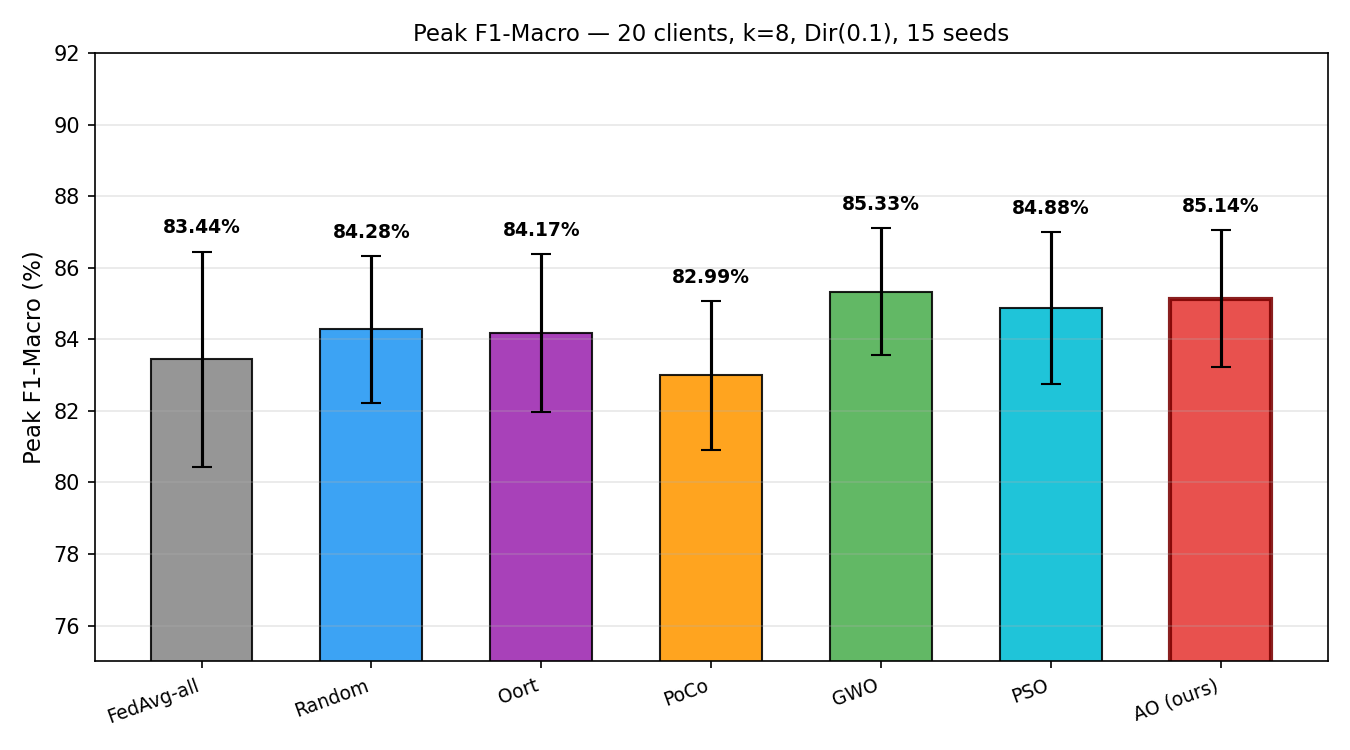
\includegraphics[width=\columnwidth]{figures/bar_peak_f1.png}
\caption{Peak F1-macro (mean $\pm$ std, 15 seeds) for each method.}
\label{fig:barf1}
\end{figure}

\subsection{Convergence Behavior}
\begin{figure}[t]
\centering
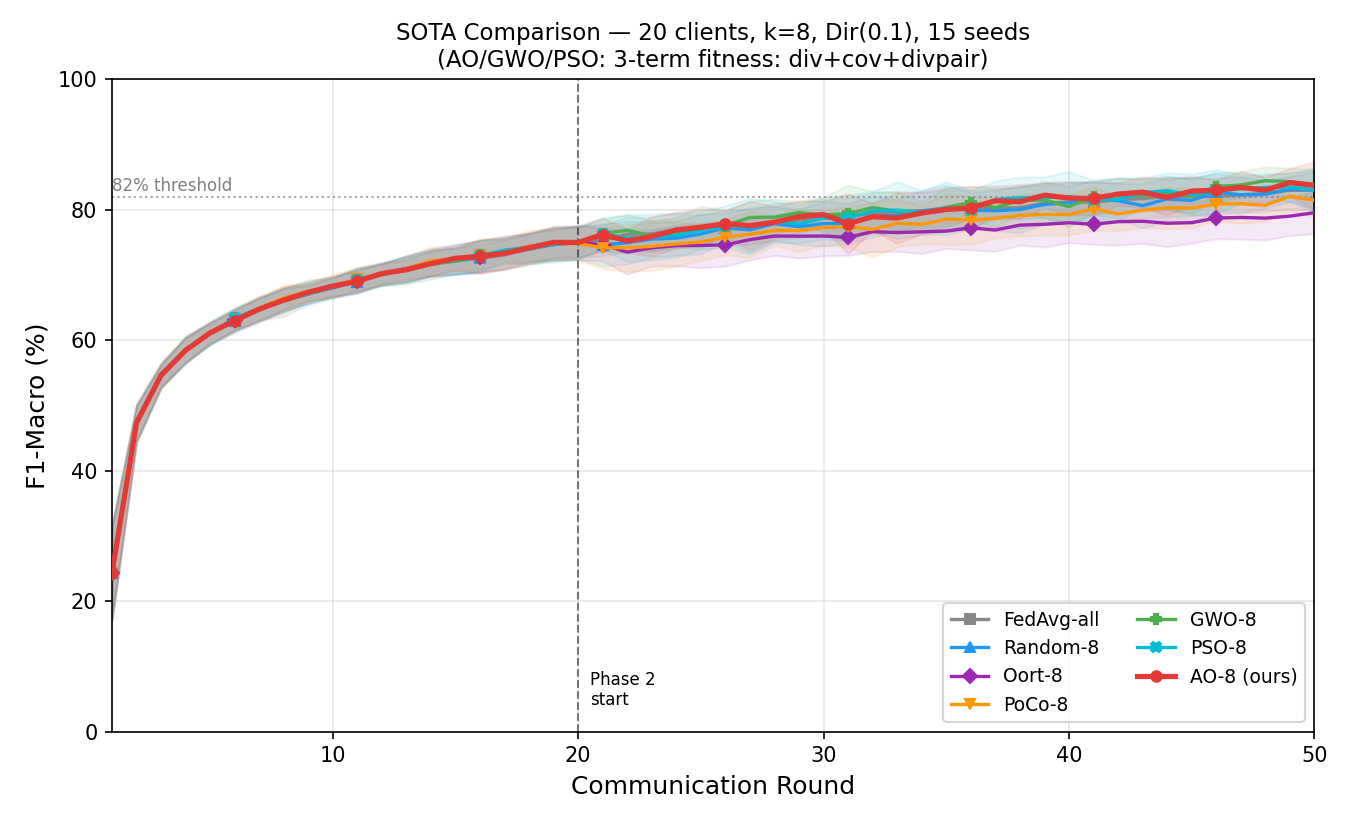
\includegraphics[width=\columnwidth]{figures/convergence_curves.png}
\caption{Mean F1-macro across rounds (7 methods, 15 seeds; shaded $=\pm1$ std). Phase-2 selection begins at round 21.}
\label{fig:convergence}
\end{figure}
In Fig.~\ref{fig:convergence}, Oort trails the remaining six trajectory-plotted methods from round 21 onward, with wider variance bands attributable to three convergence failures (3/15 seeds capped at round 50). All methods are indistinguishable during warmup (rounds 1--20), confirming that the separation is caused by the selection strategy, not by initialization. FedAvg-all's three failures (3/15) may reflect sensitivity to client drift under severe non-IID conditions \cite{zhao2018noniid}. Note also that after warmup, divergence statistics for clients not selected in a given phase-2 round remain stale from their most recent participation; the 20-round full-participation warmup ensures all clients enter phase 2 with current statistics, substantially mitigating this cold-start effect.

\begin{figure}[t]
\centering
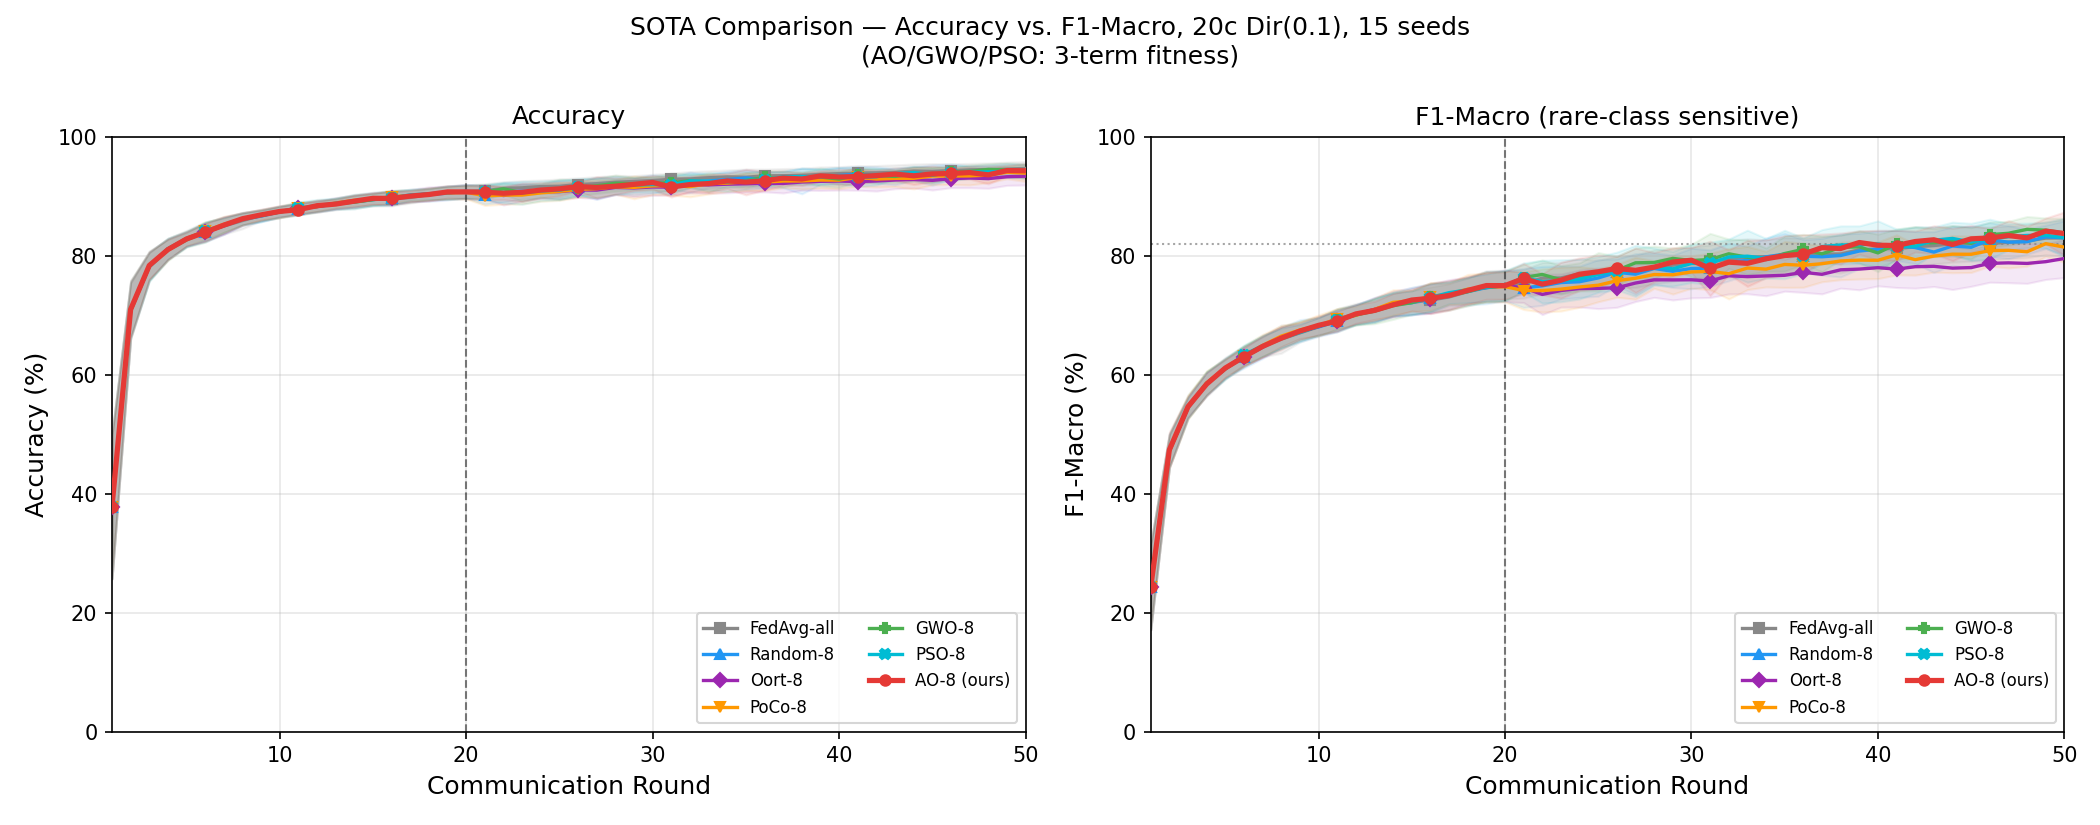
\includegraphics[width=\columnwidth]{figures/accuracy_vs_f1_dual_panel.png}
\caption{Accuracy (left) vs.\ F1-macro (right) across rounds (7 methods, 15 seeds).}
\label{fig:accf1}
\end{figure}
Accuracy masks the performance differences that F1-macro reveals. As shown in Fig.~\ref{fig:accf1}, all seven trajectory-plotted methods converge into an indistinguishable accuracy band (90--95\%), while F1-macro exposes clear separation, most strikingly for Oort. Table~\ref{tab:accf1gap} quantifies this masking effect using \emph{final-round} performance (in contrast to the peak values reported in Table~\ref{tab:sota}): every method exhibits a 10.3--13.8 percentage-point gap between accuracy and F1-macro at convergence, with Oort recording the largest gap (13.84 pp) and GWO the smallest (10.34 pp).

\begin{table}[t]
\centering
\caption{Final-round Accuracy vs.\ F1-Macro (mean, 15 seeds; DivFL and Greedy-8 excluded due to convergence failures, see Section~IV-B).}
\label{tab:accf1gap}
\begin{tabular}{lccc}
\toprule
Method & Accuracy & F1-Macro & Gap \\
\midrule
FedAvg-all & 94.67\% & 83.00\% & 11.67pp \\
Random & 94.28\% & 83.00\% & 11.28pp \\
Oort & 93.36\% & 79.53\% & 13.84pp \\
PoCo & 93.88\% & 81.43\% & 12.45pp \\
GWO & 94.17\% & 83.82\% & 10.34pp \\
PSO & 94.24\% & 83.03\% & 11.21pp \\
AO & 94.27\% & 83.71\% & 10.56pp \\
\bottomrule
\end{tabular}
\end{table}

\subsection{k-Sensitivity Analysis}
The primary comparison uses $k=8$, fixed prior to any comparative experimentation; this section confirms that conclusions are not an artefact of that choice. The main-comparison result holds across every tested $k$ value (Table~\ref{tab:ksens}). PoCo collapses at $k=10$ and $k=12$ (4/5 failures); Oort shows 0--2 failures per cell with proper training-loss utility. AO significantly outperforms Oort at $k=12$ ($p=0.031$, $d=0.83$), with a borderline trend at $k=6$ ($p=0.063$); differences at other $k$ values are not significant. AO significantly outperforms PoCo at $k\geq8$ ($p=0.031$). No significant advantage over GWO or PSO is observed at any $k$, confirming that all three metaheuristic instantiations are interchangeable solvers of the same fitness function. 
\begin{table}[t]
\centering
\caption{k-Sensitivity: Rds$\to$82\% (5 seeds per cell; failures in parentheses). $^*p=0.031$ vs.\ AO, one-sided Wilcoxon.}
\label{tab:ksens}
\footnotesize
\setlength{\tabcolsep}{3pt}
\begin{tabular}{lccccc}
\toprule
Method & $k=4$ & $k=6$ & $k=8$ & $k=10$ & $k=12$ \\
\midrule
FedAvg-all & 41.5 (3) & 42.3 (2) & 38.0 (2) & 40.0 (2) & 39.0 (2)$^*$ \\
Random     & 38.4 (0) & 38.6 (0) & 41.5 (1) & 37.3 (2) & 40.0 (1)$^*$ \\
Oort       & 43.6 (2) & 41.6 (1) & 39.4 (0) & 42.2 (0) & 44.0 (1)$^*$ \\
PoCo       & 44.0 (1) & 41.8 (1) & 42.5 (1)$^*$ & 41.0 (4)$^*$ & 34.0 (4)$^*$ \\
GWO        & 38.4 (0) & 35.2 (0) & 35.8 (1) & 36.2 (0) & 37.8 (1) \\
PSO        & 40.0 (1) & 34.2 (1) & 38.8 (0) & 37.2 (0) & 34.0 (1) \\
\textbf{AO} & \textbf{35.2 (1)} & \textbf{37.4 (0)} & \textbf{38.2 (0)} & \textbf{39.0 (0)} & \textbf{37.8 (0)} \\
\bottomrule
\end{tabular}
\end{table}

\subsection{Non-IID Sensitivity}
Table~\ref{tab:noniid} reports peak F1-macro and convergence failures across three Dirichlet heterogeneity levels. The three metaheuristic instantiations (AO, GWO, PSO) consistently cluster at the top of the ranking across all three distributions, while DivFL exhibits 5/5 convergence failures at Dir(0.1) and Oort 2/5, confirming that per-client and greedy-diversity methods degrade systematically under severe non-IID conditions. Notably, uniform random selection numerically outperforms both Oort and DivFL across all three distributions (not formally tested at $n=5$); this pattern is consistent with the hypothesis that per-client utility scoring introduces harmful selection bias under high participation rates (40\%) and severe non-IID conditions, a regime that differs markedly from the large-scale, low-participation settings in which these methods were originally validated \cite{lai2021oort, balakrishnan2022divfl}. AO significantly outperforms DivFL at Dir(0.5) ($p=0.031$, $d=0.833$), extending the head-to-head finding of Table~\ref{tab:sota} to a second heterogeneity level. AO records isolated failures in this 5-seed sweep (1/5 at Dir(0.1), 2/5 at Dir(0.05)), indicating that the zero-failure result of Table~\ref{tab:sota} reflects a strong tendency rather than a guarantee at extreme non-IID levels.

\begin{table}[t]
\centering
\footnotesize
\caption{Non-IID sensitivity: Peak F1-macro (\%, mean$\pm$std, 5 seeds per cell; failures in parentheses). $^*p=0.031$ vs.\ AO at Dir(0.5), one-sided Wilcoxon.}
\label{tab:noniid}
\setlength{\tabcolsep}{3pt}
\begin{tabular}{lccc}
\toprule
Method & \makecell{Dir(0.5)\\Moderate} & \makecell{Dir(0.1)\\Severe} & \makecell{Dir(0.05)\\Extreme} \\
\midrule
\textbf{AO (ours)} & \textbf{86.2$\pm$1.1 (0/5)} & 83.6$\pm$1.4 (1/5) & 84.7$\pm$2.4 (2/5) \\
PSO                 & 85.9$\pm$1.4 (0/5) & \textbf{84.7$\pm$0.6 (0/5)} & \textbf{85.1$\pm$1.9 (1/5)} \\
GWO                 & 85.3$\pm$1.3 (0/5) & 83.2$\pm$1.2 (1/5) & 84.9$\pm$2.2 (0/5) \\
Random              & 85.7$\pm$1.2 (0/5) & 82.7$\pm$0.8 (1/5) & 84.3$\pm$1.5 (1/5) \\
PoCo                & 85.4$\pm$0.8 (0/5) & 81.6$\pm$0.7 (3/5) & 82.7$\pm$2.2 (2/5) \\
DivFL$^*$           & 83.3$\pm$1.3 (2/5) & 80.1$\pm$1.0 (5/5) & 82.0$\pm$1.5 (4/5) \\
Oort                & 80.4$\pm$10.0 (1/5) & 82.5$\pm$1.5 (2/5) & 83.7$\pm$1.4 (1/5) \\
\bottomrule
\end{tabular}
\end{table}

\subsection{Client Selection Fairness}
All three metaheuristic optimizers converge on the same high-value clients, producing broadly similar per-client selection profiles (selection frequency std$=0.153$, $0.138$, $0.143$ for AO, GWO, and PSO respectively), consistent with their shared fitness landscape.

\subsection{Fitness-Function Term Ablation}
Model divergence emerges as the primary driver of the fitness function's effectiveness. Table~\ref{tab:ablation} reports an ablation in which each term of $F(S)$ is zeroed in turn across the same 15 seeds as Table~\ref{tab:sota}.

\begin{table}[t]
\centering
\caption{Fitness-function term ablation: AO, $k=8$, Dir(0.1), 15 seeds. $p$: one-sided Wilcoxon (full converges faster than ablated).}
\label{tab:ablation}
\footnotesize
\setlength{\tabcolsep}{3pt}
\begin{tabular}{lcccccc}
\toprule
Condition & Peak F1 & Rds$\to$82\% & Never & $p$ & $r$ & $d$ \\
\midrule
Full $F(S)$          & 85.14\% & 36.8 & 0/15 & ---   & ---   & ---   \\
No div\;[$\alpha{=}0$]      & 83.32\% & 35.6 & 3/15 & 0.164 & 0.475 & 0.253 \\
No cov\;[$\beta{=}0$]       & 84.91\% & 37.1 & 2/15 & 0.051 & 0.558 & 0.423 \\
No div$_{pair}$\;[$\lambda{=}0$] & 85.14\% & 36.2 & 1/15 & 0.462 & 0.150 & 0.024 \\
\bottomrule
\end{tabular}
\end{table}

Removal of divergence ($\alpha{=}0$) produces the largest degradation: $-1.82\%$ F1 and three additional convergence failures, medium effect ($r=0.475$, $d=0.253$), though non-significant at $n=15$. Removal of coverage ($\beta{=}0$) approaches significance ($p=0.051$, $r=0.558$). Removal of pairwise diversity ($\lambda{=}0$) yields no measurable change ($p=0.462$, $d=0.024$): at this effect size, 80\% power would require several thousand seeds. Geometrically, $\text{cov}(S)$ captures binary class presence while $\text{div}_{pair}(S)$ additionally penalizes similar class-proportion vectors, making them complementary with no measurable F1 penalty when retained. The ablation indicates divergence as the primary driver, coverage as secondary regularization, and pairwise diversity as a theoretically motivated geometric complement below the $n=15$ detection threshold. Although $\text{div}(S)$ is itself additive, its interaction with the set-level $\text{cov}(S)$---evaluated via the set union $\bigcup_{i\in S}\mathcal{C}_i$ and therefore irreducibly collective---under subset-level metaheuristic search is what per-client ranking cannot replicate: Greedy-8, which optimizes the same per-client divergence and coverage signals without subset-level evaluation, collapses to 80.90\% with 6/15 failures (Table~\ref{tab:sota}).


\section{Conclusion}

A combinatorial subset-scoring framework for FL client selection is introduced, replacing per-client scalar utility scoring with a three-term composite fitness function that captures collective model divergence, class coverage, and pairwise inter-client diversity. Evaluated on CCCS-CIC-AndMal-2020 under severe Dir(0.1) non-IID partitioning across 20 clients and 12 malware families, the framework achieves zero convergence failures across 15 seeds with statistically significant convergence improvements over Oort ($p=0.0014$, $d=0.77$) and PoCo ($p=0.046$, $d=0.44$). Validation across three structurally distinct metaheuristic instantiations (AO, GWO, PSO) of the identical fitness function confirms that the formulation, not the optimizer, drives the improvements. An ablation study suggests divergence as the likely primary contributing term, though results are non-significant at $n=15$. Future work includes scaling to larger client populations, incorporating communication and computational overhead as explicit fitness-function terms, and extending comparisons to correlation-aware methods such as FedCor \cite{tang2022fedcor} and RL-based scheduling methods such as FAVOR \cite{wang2020favor}.

\bibliographystyle{IEEEtran}
\begin{thebibliography}{99}

\bibitem{mcmahan2017}
B. McMahan, E. Moore, D. Ramage, S. Hampson, and B. A. y Arcas, ``Communication-efficient learning of deep networks from decentralized data,'' in \emph{Proc. 20th Int. Conf. Artif. Intell. Stat. (AISTATS)}, Fort Lauderdale, FL, USA, Apr. 2017, pp. 1273--1282.

\bibitem{bonawitz2019scale}
K. Bonawitz \emph{et al.}, ``Towards federated learning at scale: A system design,'' in \emph{Proc. 2nd Conf. Mach. Learn. Syst. (MLSys)}, Stanford, CA, USA, 2019.

\bibitem{lai2021oort}
F. Lai, X. Zhu, H. V. Madhyastha, and M. Chowdhury, ``Oort: Efficient federated learning via guided participant selection,'' in \emph{Proc. 15th USENIX Symp. Oper. Syst. Des. Implement. (OSDI)}, Jul. 2021, pp. 19--35.

\bibitem{cho2022poco}
Y. J. Cho, J. Wang, and G. Joshi, ``Towards understanding biased client selection in federated learning,'' in \emph{Proc. 25th Int. Conf. Artif. Intell. Stat. (AISTATS)}, Valencia, Spain, 2022.

\bibitem{fang2023fedriod}
T. Fang \emph{et al.}, ``Comprehensive Android malware detection based on federated learning architecture,'' \emph{IEEE Trans. Inf. Forensics Security}, vol. 18, pp. 3977--3990, 2023.

\bibitem{smmarwar2024review}
S. K. Smmarwar, G. P. Gupta, and S. Kumar, ``A comprehensive review of malware detection approaches using machine learning and deep learning,'' \emph{Telematics Inf. Rep.}, vol. 13, p. 100122, 2024.

\bibitem{abualigah2021aquila}
L. Abualigah, A. Diabat, S. Mirjalili, M. A. Elaziz, and A. H. Gandomi, ``The Aquila Optimizer: A novel meta-heuristic optimization algorithm,'' \emph{Comput. Ind. Eng.}, vol. 157, p. 107250, 2021.

\bibitem{mirjalili2014gwo}
S. Mirjalili, S. M. Mirjalili, and A. Lewis, ``Grey wolf optimizer,'' \emph{Adv. Eng. Softw.}, vol. 69, pp. 46--61, 2014.

\bibitem{kennedy1995pso}
J. Kennedy and R. Eberhart, ``Particle swarm optimization,'' in \emph{Proc. IEEE Int. Conf. Neural Netw.}, Perth, Australia, 1995, pp. 1942--1948.

\bibitem{balakrishnan2022divfl}
R. Balakrishnan, T. Li, T. Zhou, N. Himayat, V. Smith, and J. Bilmes, ``Diverse client selection for federated learning via submodular maximization,'' in \emph{Proc. Int. Conf. Learn. Represent. (ICLR)}, 2022.

\bibitem{tang2022fedcor}
M. Tang, X. Ning, Y. Wang, J. Sun, Y. Wang, Y. Chen, and Y. Lin, ``FedCor: Correlation-based active client selection strategy for heterogeneous federated learning,'' in \emph{Proc. IEEE/CVF Conf. Comput. Vis. Pattern Recognit. (CVPR)}, 2022.

\bibitem{wang2020favor}
H. Wang, Z. Kaplan, D. Niu, and B. Li, ``Optimizing federated learning on non-IID data with reinforcement learning,'' in \emph{Proc. IEEE INFOCOM}, 2020.

\bibitem{qolomany2020psofl}
B. Qolomany, K. Ahmad, A. Al-Fuqaha, and J. Qadir, ``Particle swarm optimized federated learning for industrial IoT and smart city services,'' in \emph{Proc. IEEE Global Commun. Conf. (GLOBECOM)}, 2020.

\bibitem{yamany2024gwofl}
W. Yamany, M. Keshk, N. Moustafa, and B. Turnbull, ``Swarm optimization-based federated learning for the cyber resilience of Internet of Things systems against adversarial attacks,'' \emph{IEEE Trans. Consum. Electron.}, vol. 70, no. 1, pp. 1359--1369, Feb. 2024.

\bibitem{cicandmal2020}
A. Rahali, A. H. Lashkari, G. Kaur, L. Taheri, F. Gagnon, and F. Massicotte, ``DIDroid: Android malware classification and characterization using deep image learning,'' in \emph{Proc. 10th Int. Conf. Commun. Netw. Secur. (ICCNS)}, Tokyo, Japan, 2020, pp. 70--82.

\bibitem{keyes2021entropLyzer}
D. S. Keyes, B. Li, G. Kaur, A. H. Lashkari, F. Gagnon, and F. Massicotte, ``EntropLyzer: Android malware classification and characterization using entropy analysis of dynamic characteristics,'' in \emph{Proc. IEEE Reconcil. Data Anal., Autom., Privacy, Secur. (RDAAPS)}, 2021.

\bibitem{khan2024swarm}
K. Khan and W. Goodridge, ``Swarm intelligence-driven client selection for federated learning in cybersecurity applications,'' arXiv preprint arXiv:2411.18877, Nov. 2024.

\bibitem{bendriss2024gwo}
M. Ben Driss, E. Sabir, H. Elbiaze, A.~B. Diallo, and M. Sadik, ``A green multi-attribute client selection for over-the-air federated learning: A grey-wolf-optimizer approach,'' \emph{ACM Trans. Model. Perform. Eval. Comput. Syst.}, 2024.

\bibitem{li2024survey}
J. Li, T. Chen, and S. Teng, ``A comprehensive survey on client selection strategies in federated learning,'' \emph{Comput. Netw.}, vol. 251, p. 110663, 2024.

\bibitem{zhao2018noniid}
Y. Zhao, M. Li, L. Lai, N. Suda, D. Civin, and V. Chandra, ``Federated learning with non-IID data,'' \emph{arXiv preprint} arXiv:1806.00582, 2018.

\bibitem{hsu2019dirichlet}
T.-Y. Hsu, H. Qi, and M. Brown, ``Measuring the effects of non-identical data distribution for federated visual classification,'' \emph{arXiv preprint} arXiv:1909.06335, 2019.

\bibitem{nemeth2025feddiverse}
G. D. N\'{e}meth, E. Fan\`{i}, Y. J. Ng, B. Caputo, M. \'{A}. Lozano, N. Oliver, and N. Quadrianto, ``FedDiverse: Tackling data heterogeneity in federated learning with diversity-driven client selection,'' in \emph{Proc. 3rd IEEE Int. Conf. Federated Learning Technol. Appl. (FLTA)}, 2025.

\bibitem{wu2025fedcsga}
J. Wu, H. Ji, J. Yi, and L. Liu, ``Optimizing client selection in federated learning based on genetic algorithm,'' \emph{Cluster Comput.}, vol. 28, p. 400, 2025.

\bibitem{panimalar2026fedgenblk}
S. P. Panimalar and S. Gunasundari, ``Robust federated learning for cloud environments using evolutionary optimization and blockchain,'' \emph{Sci. Rep.}, vol. 16, p. 4202, 2026.

\bibitem{zhang2023dpp}
Y. Zhang, C. Xu, H. H. Yang, X. Wang, and T. Q. S. Quek, ``Determinantal point process-based client selection for federated learning with non-IID data,'' in \emph{Proc. IEEE Int. Conf. Acoust., Speech Signal Process. (ICASSP)}, Rhodes Island, Greece, 2023.

\end{thebibliography}

\end{document}
